\documentclass{mm2}
\usepackage{bbm}
\usepackage{amsmath}
\usepackage{bbold}
\usepackage{multicol}


% FILL THIS WITH YOUR CIS USERNAME
\cisid{bzqs27} 
\title{Digital Communications - Huffman Encoding}

\begin{document}
\section{Executing the Program(s)}
\subsection{Encoding and Decoding}
In order to execute the program you must have python3 installed, executing encoding and decoding is relatively similar.

\subsubsection{Execution Method: Using the command line}
\begin{enumerate}
\item Open terminal/commandprompt (or whatever CLI you are using).
\item Input a line of the form: python3 'full path and name of encoder.py' 'full path and name of text file you're compressing'
\item To decode do the same but the line will be of the form: python3 'full path and name of decoder.py' 'full path and name of hc you're decompressing'\\
E.g. python3 /Users/harryrichards/Desktop/encoder.py /Users/harryrichards/Desktop/fname.txt
\end{enumerate}

\section{Implementation}
\subsection{Huffman Encoding (Implementation)}
If the steps for executing the encoding program have been followed correctly then the program will have been provided with the a file to perform the huffman encoding on and the following will occur. The  file is read to a string, when doing so we specify the condition newline = '', this ensures new line characters are interpreted in the form that they were written regardless of the platform you are reading the file on. If we were to omit this then new line characters are interpreted differently dependent on the platform you are using i.e. Python would interpret the newline as $\backslash n$ on a unix machine but would interpret a newline as $\backslash r \backslash n$ on a windows machine - this will ensure the newline character in the decoded file is the same as in the file prior to encoding.\\
The next step is to form a dictionary of the form $\{ character : frequency \}$ in order to do this we iterate over each character in the file and each time the character appears we increment the value of the characters frequency by 1, the dictionary is then sorted by frequency in descending order, this will simplify implementing the building of the tree.\\
In order to form a tree we will need to be able to form a node and relate it to other nodes, this relationship shall be a node being the parent of other nodes, more specifically a parent node is capable of having both left and right children. In fact a parent node is required to have both left and right child in this implementation. Thus we form a class which specifies the characteristics of a node. A node is required to have a frequency, as well as a character ( we often set this to 'None' in our implementation). A node is capable of have a code, a left child and a right child as attributes (initially each nodes code is an empty string, and their left and right children are 'None'). A list is instantiated in which we will store nodes of the tree. For each character in the dictionary, we create a node, setting the character of the node to be the character in question, and the frequency of the node to be the corresponding frequency. We now have a list of independent 'base nodes' for each character. \\
From here we can begin to form our tree, and find the root node. In order to build the tree we use the list of the current nodes, and while this list contains more than one node ($\text{while } len(nodes)>1:$), we sort the list in descending order (with respect to frequency),and 'pop off' the two nodes with least frequency. A new node (instance of node class) is formed with frequency that is the sum of these two frequencies, and the two nodes we 'popped off' are set as its left and right children. The new node is appended to this list of nodes. This process is repeated over and over again until we reach a point when the list of nodes has length 1, this indicates that there is only one node in the list and this node must be the root node, this is returned.\\
From the root node we are able to access every other node somehow, and thus we can use this to formulate the codes of our initial 'base nodes', and hence these will be the codes of the characters correspodning to these nodes. Due to the manner in which we acquired the root node (the aforementioned while loop $\text{while } len(nodes)>1:$), the root node will be returned as 'None' if there is only one character in the file. Thus I implemented a special case for this in which I set the character code for this singular character equal to '0' as this is the smallest code possible. \\
However, if the root node is not 'None' we can use it to formulate codes for each of the characters. We must first make a list containing only the root node, this list is passed into a method and each node in the list is iterated over (initially just the root node), if the node has a value for character (that is not equal to None) then an element of the form 'node character : node code' is added to a dictionary that stores each character and that characters code. However, if the node does not have a character then we know this node must have children. If the node has a left child, we concatenate a '0' onto the value of the left childs code, and if the node has a right child we concatenate a '1' onto right childs code. We add all children to a list of new nodes, and repeat this process for each of the nodes in the nodes list. We then call the function we are currently using recursivel and pass in the new nodes list, by doing so we will continually find the codes of child nodes until we have found the codes of all the nodes in the tree, at which point we will have a dictionary relating each character to a code.\\
I now instantiate an array in which I will append the codes of each of the characters in the current file string. For each character in the file string, I append the code corresponding to this character to the array. When this is complete I use the .join method to join the elements of the array to form the new encoded file string. The reason behind appending the elements to an array and then joining the array to form a string rather than immediately concetanating a string is that the appending to a list/array is usually much quicker than concetanating elements to a string, and either after using .join method after experimenting I found this was quicker.\\
Now we have the new file string which is a bitstring, in order to compress the file I must split this into bytes, so I now make sure that the new file string length is a multiple of 8. To do so I calculate $ length\, of \,bistring - length \, of \, bitstring \, mod \,8$ and concatenate that amount of $0s$ to the bitstring. Then I instantiate a byte array, and begin iterating over the new bitstring taking slices of length 8 and appending the integer value of the byte forme to the byte array until we have reached the end of the bitstring.\\
Now, we have acquired all of the necessary data in order to write (create) the huffman encoded (compressed) file. We now create a file with the same name as the original file we opened with the replacing the .txt extension with .hc. The program writes to this file in binary, pickle simply dumps the dictionary, number of extra zeros and file byte array to the (new) compressed file.
\subsection{Huffman Decoding (Implementation)}
If the steps for executing the program are followed correctly then the program will be provided with the filename of the file that we wish to decode (from the encoded .hc form to the original .txt form). We can first open the file (in read binary mode) and use the pickle.load(file) 3 times separately, saving the result to variables and it will provide us with the 3 pickle dumps that were produced in the encoding phase (these are the dictionary, number of extra zeros and byte array respectively). This will provide us with the dumps in the order they were dumped.\\
Now that the necessary information has been loaded we can invert the dictionary that we just loaded, we could have dumped the inverted dictionary instead but I felt this order was more logical. Inverting the dictionary this should save time when accessing the character corresponding to a key later.\\
Now I instantiate an array which I will store elements of a string in, with the same thought as above this should allow me to append elements of the string to the array quickly and then perform one large but (net) quicker string concetanation with all the elements at the end in order to form our bitstring. When forming this bitstring we iterate through each byte in the bye array that we loaded. We convert each byte to binary, and trim the first 2 digits (as they will be '0b' that were added by default when we first added the elements to a byte array), I also use the zfill function ($byte = bin(originalByte)[2:].zfill(8)$) on the byte in order to  make sure that each byte is 8 bits long as they were when I wrote them to the file, as the byte array deems 0s prior to the first 1 as redundant as it says nothing about the value, however it is essential if we wish to form the original bitstring correctly. When each byte has been added to the array, the .join method is used to form the original bitstring that we arrived at after encoding. I trim the extra zeros *that we added during encoding) from the end of the bitstring, as the extra zeroes were not in the bitstring that we encoded and we simply added them so we could store the encoded string conveniently as bytes - thus it is important the number of extra zeroes is stored and loaded.\\
Now we have the original bitstring we encoded to, we simply need to check if it starts with a key of the inverted dictionary, and if it does we will add this key to the decoded file string and we will repeate this until we have decoded the full string (ignoring bits that were previously accounted for). In order to do this as quickly as possible I implemented the following function. Instantiate an array (to store characters of the original file string) that we will later join, instantiate an empty string (let us call this the temp string). For each character in the bitstring (i.e. a 0 or 1) concentante the character to the temp string, if the temp string is a key in the dictionary then append the value associated with the key to the original text array and set the temp string to blank, if not then simply proceed to concetanate the next character. Eventually this will cause the original text array to contain every character in the original file. Once each character has been iterated over return the elements of the array joined together as a string. Write this to a file with the same file name as the .hc file we are decoding except replace the extension .hc with .txt. This should be the same as the txt file prior to encoding.
\subsection{Further Design Choices}
\subsubsection{Using arrays/lists instead of strings and limiting loop usage}
After looking into arrays I found it was much quicker to append an item to an array/list than it is to concetanate a string version of the item to a string. However, I felt that when using the .join method on the array to form a string from the elements of the array that we are essentially performing one long string concetanation so any time saved by using an array/list would be lost here. However after testing this multiple times I found that generally the use of arrays and .join were faster than direct string concetanation. Ultimately I opted for this option as it seemed quicker in practice and replaced a lot of my string concatenation with list appendage in order to optimise speed of both programs. I also limited the number of loops that I used in order to make sure that I wasn't iterating over things unnecessarily, this improved speed.
\subsubsection{Storing the dictionary}
I assumed that when decoding the file we would need to access the dictionary that related each character to its code from the .hc file somehow, and that it wasn't acceptable to simply write the dictionary to a separate file or store it to a variable or something of this sort. When researching I found that there were multiple methods of writing the dictionary, for example one which required writing 2 bytes to the file (the character stored and the length of its bytes) followed by the code for the character (for each character), and that when decoding the encoded this would be read first in order to re-form the dictionary. I felt this used an large amount of bytes unnecessarily compared to other methods (especially large files), as well as parsing it to a dictionary would likely to take a large amount of time when decoding compared to said methods thus I decided against it.\\
After much thought I decided to try using the in-built python libraries pickle or json. When comparing the two on some of my own test files I found that json used far less data, and pickle was marginally faster on some of the larger files. Figures (\ref{fig:picklejson1}) and (\ref{fig:picklejson2}) are comparisons of the size of pickle dumps in comparison to json dumps, and the time taken to load for both JSON and Pickle files.
\begin{figure}[ht]
\minipage{0.48\textwidth}
  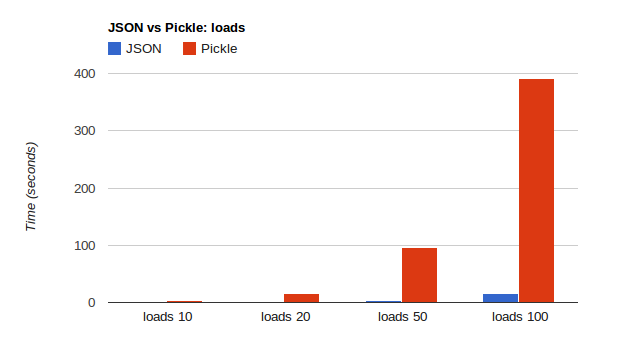
\includegraphics[width=\linewidth]{figures/picklejson1.png}
  \caption{A comparsion of time taken to load for JSON and Pickle.}\label{fig:picklejson1}
\endminipage\hfill
\minipage{0.48\textwidth}%
  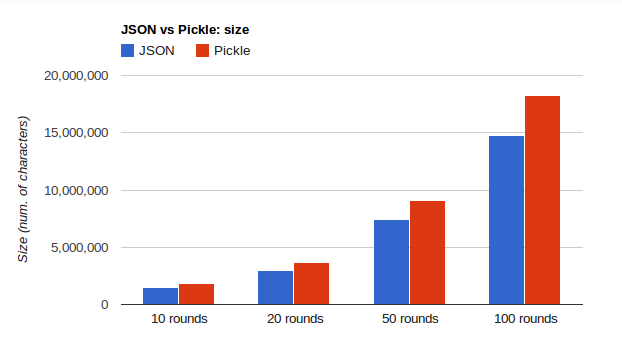
\includegraphics[width=\linewidth]{figures/picklejson2.png}
  \caption{A comparsion of time taken to load for JSON and Pickle.}\label{fig:picklejson2}
\endminipage
\end{figure}
As we can see JSON seems to optimise the amount of compression where as pickle seems to optimise runtime. However, the fact pickle is more convenient for writing to a file with binary format and the data will only be used with python which seems to nullify many of JSONs benefits, also JSON can't handle arbitrary objects as pickle can and this made decoding the file more time consuming and more difficult generally.
\section{Performance Analysis}
\subsection{Encoder and Decoder running time}
\begin{figure}[ht]
\minipage{0.48\textwidth}
  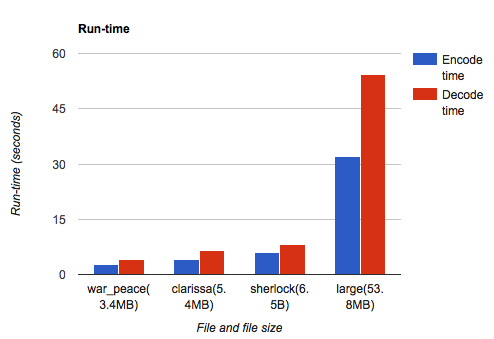
\includegraphics[width=\linewidth]{figures/timegraph.png}
  \caption{A graph comparing of time taken to encode and decode for different files.}\label{fig:timegraph}
\endminipage\hfill
\minipage{0.48\textwidth}%
  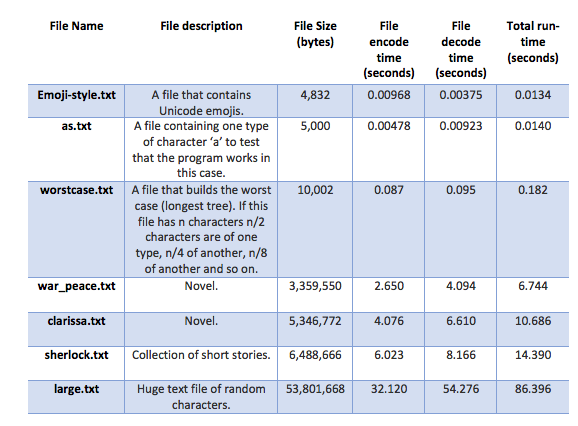
\includegraphics[width=\linewidth]{figures/timetable.png}
  \caption{A table comparing of time taken to encode and decode for different files.}\label{fig:timetable}
\endminipage
\end{figure}
The above displays the encoding and decoding run-times provided by the time library in python. As you can see for large text files (several MB) the total run-time ranges from around 6 seconds to around 14 seconds. For a huge 54 MB text file the run-time is around 1 minute 26 seconds and for a relatively small text file the run-time is around $\frac{1}{100}^{th}$ of a second, almost instantaneous. Each of these files where designed in specifically to test a certain aspect of the encoding, for instance the 'emoji' file whilst being small tests how the encoding copes when presented with unicode. I believe these are all more than reasonable times to wait and for real-world use this is very convenient. The worst case text file has a run-time of the around 0.182 seconds, this is because the file was designed in way that the huffman tree produced would be as large as possible (by having $\frac{1}{2}$ of the characters of one type $\frac{1}{4}$ of another $\frac{1}{8}$ of another and so on), if I were to increase the number of characters I used then I could create a very large tree that may take a while to traverse under these conditions however I would consider this more a limitation of the huffman algorithm than my implementation. Clearly files with more bits take longer to compress but also if we compare the 'emoji' file and the 'as' file we see that files with more repetition can be compressed much faster than those that lack repetition.
\subsection{Compression Ratio(s)}
Below we see Figures (\ref{fig:compressiongraph}) and (\ref{fig:compressiontable})displaying the original sizes of some of the files that I tested my compression on, along with their size after compression and the compression ration which I defined as $compression \, ratio = \frac{encoded \, file \, size}{original \, file \, size}$ in each case.
\begin{figure}[ht]
\minipage{0.48\textwidth}
  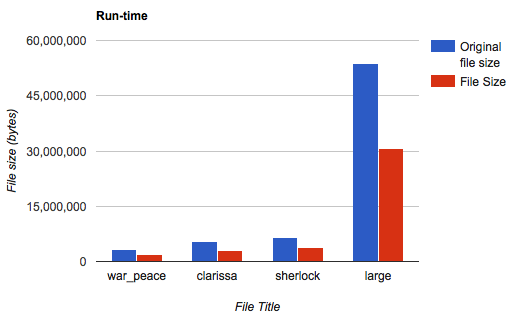
\includegraphics[width=\linewidth]{figures/compressiongraph.png}
  \caption{A graph comparing original file size and encoded file size on various text files.}\label{fig:compressiongraph}
\endminipage\hfill
\minipage{0.48\textwidth}%
  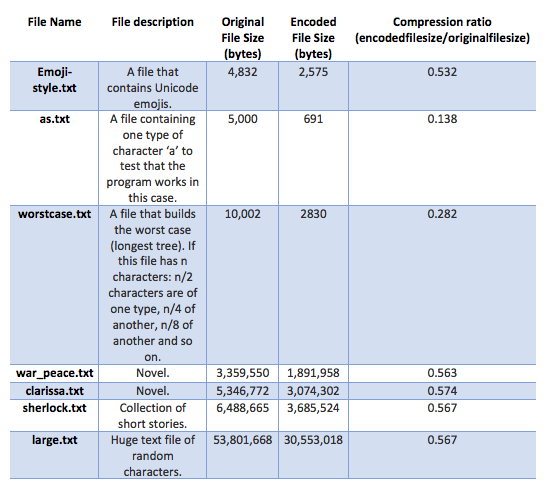
\includegraphics[width=\linewidth]{figures/compressiontable.png}
  \caption{A table comparing original file size and encoded file size on various text files.}\label{fig:compressiontable}
\endminipage
\end{figure}

We see that most larger files tend to compress to around $56\%$ of their original size, I believe this is a very solid amount of compression however it is limited by my use of pickle to store the data, however I believe this is still justified as we can see it works quickly from Figures (\ref{fig:timegraph}) and (\ref{fig:timetable}). Obviously the nature of the huffman algorithm means that the more repition in a file, the more succesful the compression will be and the figures (\ref{fig:compressiongraph}) and (\ref{fig:compressiontable}) exemplify this as we see that in a file containing only one character the compression is around $90\%$ and would be even more impressive if we stored the dictionary using json in this case.

\section{Performance Improvement and Conclusion}
\subsection{Limitations}
Clearly we see that the huffman algorithm is succesful in compressing simple text files, this is indisputable. However, my implementation (and the algorithm) is limited in some sense as the compression we can achieve is limited by the number of bitstrings less than 8 bits. If we have a vast number of characters such as in unicode, then we will soon exhaust all of the bitstrings less than 8 in length and at this point the algorithm will not be compressing a characters size and it may even increase it in size. If the file is altered then the entire compression process must re-occur in order to gain optimum compression. My implementation does not consider strings of characters, and this would improve compression. I also feel that the speed of the process is limited by the use of python, and in order to improve this I could implement c-extensions in python such as bitarray. Also files with no repetition or limited repetition are often not compressed due to the fact the dictionary takes up so much space.
\subsubsection{Compression Ratio}
In order to improve the compression ration I belive considering blocks of characters e.g. ab and checking how frequently this occurs would aid the compression. If I were to reattempt this I would incorporate this by considering blocks of length $n$ as this has potential to reduce an $n-byte$ bitstring to a singular bit whereas currently there is only potential to reduce a byte to a bit. I would also look into writing a function that calculates $n$, and allow the user to specify $n$ if they have a particular $n$ they wish to use (if not then calculate it). I also believe that in order to improve the compression ratio I could look into a more practical way of storing the dictionary as a json object and this would reduce the total file size, there are also most likely even better ways to store the dictionary howevery they may make it harder to deal with the file.
\subsubsection{Speed}
I believe that python and using a byte array slowed down the encoding and decoding process hugely, and that after experimenting with bitarray (a C extension) that if I were to reimplement the algorithm, using bitarray would speed up the process massively.
\subsubsection{Conclusion}
The Huffman algorithm is a really useful tool for compression of plain text files and it does well to take advantage of the repetition of characters without losing any quality in the file. However, when there is limited or no repetition it is practically useless and its doubtful it will be able to perform any kind of compression. However, as the target of compression tends to be large files it is extremely unlikely that the file will not contain any repetition and in fact I would expect it to contain a considerable amount thus huffman will work well in most cases.
\end{document}